\documentclass{magnolia}

\magtex{tex_driver={pdftex},
        tex_packages={xypic}}
\magfiche{document_nom={Cours Python sur les listes},
          auteur_nom={François Fayard},
          auteur_mail={fayard.prof@gmail.com}}
\magcours{cours_matiere={python},
          cours_niveau={mpsi},
          cours_chapitre_numero={4},
          cours_chapitre={Liste, pile, file, dictionnaire}}
\magmisenpage{misenpage_presentation={tikzvelvia},
              misenpage_format={a4},
              misenpage_nbcolonnes={1},
              misenpage_licence={non},
              misenpage_preuve={non},
              misenpage_exemple={oui},
              misenpage_prof={non}}
\maglieudiff{lieu_lycee={Aux Lazaristes},
             lieu_classe={MPSI 1},
             lieu_annee={2019--2020}}
\magprocess

\begin{document}
%BEGIN_BOOK
\hfill\includegraphics[width=0.45\textwidth]{../../Commun/Images/python-cours-organisation-gaston}

\magtoc

\bigskip

Si l'on dispose d'une collection ordonnée d'objets comme des relevés de température effectués
chaque jour d'un mois ou une liste de vêtements, il est naturel de les regrouper à l'aide d'un objet
informatique que l'on appelle \emph{collection}. Un peu comme il existe différentes manières de
ranger ses pantalons, il existe différentes façons d'organiser une collection dans
la mémoire de l'ordinateur. En informatique, une telle organisation est appelée une
\emph{structure de données}.\\

Prenons l'exemple d'une collection de pantalons que l'on souhaite ranger dans notre placard. La manière
la plus courante de les organiser est de les placer en \emph{pile} comme ci-dessous~:
\begin{center}
\includegraphics[width=0.4\textwidth]{../../commun/images/python-cours-jeans-pile}
\end{center}
Une autre manière de les ranger est d'avoir une succession de compartiments
dans lesquels on peut ranger chaque pantalon. En informatique, une telle organisation est appelée
un \emph{tableau}.
\begin{center}
\includegraphics[width=0.3\textwidth]{../../commun/images/python-cours-jeans-tableau}
\end{center}
Chaque organisation a ses avantages et ses inconvénients~:
\begin{itemize}
\item Le tableau à l'avantage de donner un accès direct à tous les pantalons. Cependant, il ne permet
  pas d'en rajouter de nouveau.
\item La pile permet facilement d'ajouter un nouveau pantalon dans notre collection, en
  le plaçant au sommet, mais elle ne permet l'accès direct qu'au pantalon placé sur le dessus.
  Si vous souhaitez accéder soigneusement à un pantalon qui se trouve en dessous, il est
  nécessaire de dépiler un à un chaque pantalon.
\end{itemize}
Python propose une structure de données qu'il appelle \emph{liste} et qui essaie de faire la synthèse
des deux qualités essentielles des structures de données précédentes~: la possibilité d'avoir un
accès direct à chaque objet et celle d'ajouter facilement un objet en fin de collection. L'analogie la plus
proche en terme de rangement est la suivante
\begin{center}
\includegraphics[width=0.3\textwidth]{../../commun/images/python-cours-jeans-tabdyn}
\end{center}
où l'on imagine que les pantalons doivent toujours être placés sur les tiges situées les plus à gauche.

% Une \emph{structure de donnée} est une façon de ranger une collection d'objets en mémoire.
% La manière la plus élémentaire de disposer une série d'objets est de les placer côte à côte,
% dans des emplacements mémoire contigus. 

% Les programmes que nous avons écrits jusqu'à présent ne travaillaient qu'avec un nombre
% limité de valeurs. Nous avons par exemple écrit une fonction calculant le minimum de deux
% nombres flottants. Si notre algorithme doit travailler non pas avec deux nombres flottants,
% mais avec une dizaine de nombres, des milliers, voire des milliards, nous devons stocker
% cette collection de valeurs dans une \emph{structure de donnée}. Différentes méthodes
% existent pour stocker en mémoire ces données. Selon l'algorithme que l'on souhaite utiliser
% pour traiter ces données, certaines sont plus performantes que d'autres. Dans ce chapitre,
% nous allons introduire une des structures de données concrètes des plus importante en
% informatique~: \emph{le tableau dynamique}. C'est, avec la \emph{liste chainée}, la structure
% de donnée concrète le plus utilisée pour stocker une collection ordonnée d'objets. Le
% tableau dynamique est fondamental en programmation impérative alors que la liste chainée est
% fondamentale en programmation fonctionnelle. Python propose un tableau dynamique
% qu'il appele liste.

\section{Liste}

\subsection{Liste}

Une liste est une succession ordonnée de $n$ valeurs. La manière la plus simple de définir une
liste est d'énumérer ses éléments en les plaçant entre crochets et en les séparant par des virgules.
Par exemple, si l'on souhaite définir la liste des températures moyennes en France des 10 premiers jours
de juillet 2022, on écrit~:

\begin{pythoncode}
In [1]: t = [23, 25, 23, 23, 25, 24, 24, 23, 27, 22]
\end{pythoncode}
\noindent
La longueur d'une liste $t$, c'est-à-dire le nombre d'éléments qu'elle contient,
est obtenue avec \verb!len(t)!. On la notera souvent $|t|$. Si $t$ est une liste de longueur
$n$, ses éléments sont indexés de 0 à $n-1$. On imaginera un tableau possédant $n$ cases
et contenant les éléments de la collection. Voici par exemple une représentation du tableau
précédent de longueur $n=10$.
\begin{center}
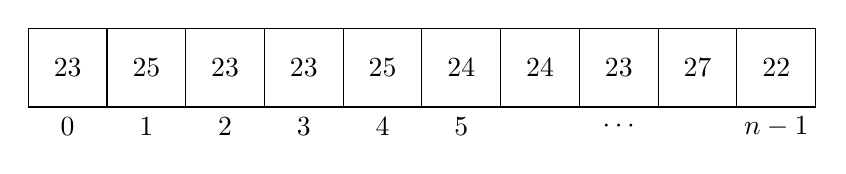
\begin{tikzpicture}
\filldraw [fill=white, draw=black] (0,0) rectangle (1,1) node[pos=.5] {23};
\filldraw [fill=white, draw=black] (1,0) rectangle (2,1) node[pos=.5] {25};
\filldraw [fill=white, draw=black] (2,0) rectangle (3,1) node[pos=.5] {23};
\filldraw [fill=white, draw=black] (3,0) rectangle (4,1) node[pos=.5] {23};
\filldraw [fill=white, draw=black] (4,0) rectangle (5,1) node[pos=.5] {25};
\filldraw [fill=white, draw=black] (5,0) rectangle (6,1) node[pos=.5] {24};
\filldraw [fill=white, draw=black] (6,0) rectangle (7,1) node[pos=.5] {24};
\filldraw [fill=white, draw=black] (7,0) rectangle (8,1) node[pos=.5] {23};
\filldraw [fill=white, draw=black] (8,0) rectangle (9,1) node[pos=.5] {27};
\filldraw [fill=white, draw=black] (9,0) rectangle (10,1) node[pos=.5] {22};
\node[] at (0.5,-0.25) {0};
\node[] at (1.5,-0.25) {1};
\node[] at (2.5,-0.25) {2};
\node[] at (3.5,-0.25) {3};
\node[] at (4.5,-0.25) {4};
\node[] at (5.5,-0.25) {5};
\node[] at (7.5,-0.25) {$\cdots$};
\node[] at (9.5,-0.25) {$n-1$};
\end{tikzpicture}
\end{center}
Il est important de remarquer que l'indice de la première case est 0 (et non 1 comme dans certains langages de programmation) et que celui de la
dernière case est $n-1$ (et non $n$). On a un accès direct à l'élément d'indice $k$ 
pour tout $k\in\interefo{0}{n}$ grâce à \verb!t[k]!. Si l'on tente d'accéder à un élément \verb!t[k]! pour $k\geq n$,
Python lève une exception qui se solde par une erreur.\\

Python permet aussi d'accéder aux éléments de la liste en les indexant \og par la fin \fg. On utilise
pour cela des indices strictement négatifs $k\in\interefo{-n}{0}$.
\begin{center}
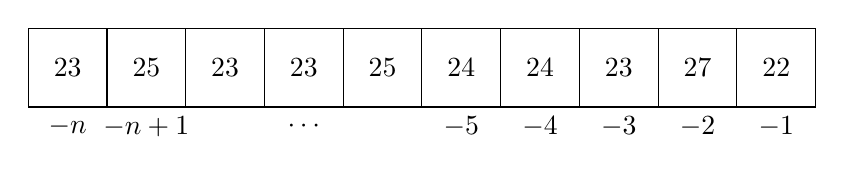
\begin{tikzpicture}
\filldraw [fill=white, draw=black] (0,0) rectangle (1,1) node[pos=.5] {23};
\filldraw [fill=white, draw=black] (1,0) rectangle (2,1) node[pos=.5] {25};
\filldraw [fill=white, draw=black] (2,0) rectangle (3,1) node[pos=.5] {23};
\filldraw [fill=white, draw=black] (3,0) rectangle (4,1) node[pos=.5] {23};
\filldraw [fill=white, draw=black] (4,0) rectangle (5,1) node[pos=.5] {25};
\filldraw [fill=white, draw=black] (5,0) rectangle (6,1) node[pos=.5] {24};
\filldraw [fill=white, draw=black] (6,0) rectangle (7,1) node[pos=.5] {24};
\filldraw [fill=white, draw=black] (7,0) rectangle (8,1) node[pos=.5] {23};
\filldraw [fill=white, draw=black] (8,0) rectangle (9,1) node[pos=.5] {27};
\filldraw [fill=white, draw=black] (9,0) rectangle (10,1) node[pos=.5] {22};
\node[] at (0.5,-0.25) {$-n$};
\node[] at (1.5,-0.25) {$-n+1$};
\node[] at (3.5,-0.25) {$\cdots$};
\node[] at (5.5,-0.25) {$-5$};
\node[] at (6.5,-0.25) {$-4$};
\node[] at (7.5,-0.25) {$-3$};
\node[] at (8.5,-0.25) {$-2$};
\node[] at (9.5,-0.25) {$-1$};
\end{tikzpicture}
\end{center}
Cependant, cette manière d'accéder aux listes est à priori proscrite aux concours. On se permettra
cependant d'utiliser la syntaxe bien pratique \verb!t[-1]! permettant d'accéder au dernier
élément d'une liste.\\

Les listes Python peuvent contenir des valeurs de types différents. Elles peuvent même contenir d'autres listes.

\begin{pythoncode}
In [2]: t = [9, 3.14159, "Hello", True, [3, 8]]
\end{pythoncode}

\noindent
Cependant, contrairement aux \verb_tuple_, l'utilisation des listes se fera essentiellement
avec des valeurs ayant le même type. Quels que soient les éléments qu'elle contient, le type d'une
liste est \verb!list!, mais dans la signature d'une fonction, on notera \verb!list['a]! pour désigner
le type d'une liste d'éléments de même type \verb!'a!.

\subsection{Parcours de liste}

Nous avons vu dans le second chapitre comment parcourir une liste. La manière la plus conventionnelle
est d'effectuer une boucle sur un entier $k$ qui va prendre successivement les indices admissibles
pour la liste. Par exemple, la fonction suivante va tester si un entier $x$ est un élément de la
liste $t$~:
\begin{pythoncodeline}
def est_present(x, t):
    """est_present(x: int, t: list[int]) -> bool"""
    for i in range(len(t)):
        if t[i] == x:
            return True
    return False
\end{pythoncodeline}
Il est cependant possible d'écrire la même fonction de manière plus concise, en itérant
non par sur les indices de la liste, mais directement sur la liste elle-même. Pour cela, on
utilise la syntaxe \og \verb!for y in t! \fg~: dans ce cas, la boucle va itérer sur les éléments
de la liste et $y$ va prendre successivement les valeurs $t_0, t_1,\ldots,t_{n-1}$. La fonction \verb!est_present! peut donc s'écrire ainsi~:
\begin{pythoncodeline}
def est_present(x, t):
    """est_present(x: int, t: list[int]) -> bool"""
    for y in t:
        if y == x:
            return True
    return False
\end{pythoncodeline}
Le fait qu'on puisse écrire \og \verb!for y in t! \fg fait de la liste \verb!t! un objet \emph{itérable}.
D'autres objets Python possèdent cette propriété~: les chaines de caractères et les tuples. La fonction
\verb!possede_un_e! vue au chapitre précédent s'écrit donc~:
\begin{pythoncodeline}
def possede_un_e(s):
    """possede_un_e(s: str) -> bool"""
    for c in s:
        if c == 'e':
            return True
    return False
\end{pythoncodeline}
Les deux styles ont chacun leurs avantages et leurs inconvénients. L'utilisation d'une liste en tant
qu'objet itérable a l'avantage de la concision, mais l'utilisation d'un indice et d'un \verb!range! est parfois nécessaire.\\

Nous avons vu dans le second chapitre des algorithmes de réduction permettant de
calculer la somme, le produit ou le maximum des éléments d'une liste. Ces algorithmes sont essentiels
et nous ne les redétaillerons pas ici. Nous allons plutôt détailler deux nouveaux algorithmes~:
l'algorithme de Horner et la méthode de recherche dichotomique dans une liste triée.

\subsubsection{Algorithme de Horner}

Les listes sont de bons candidats pour représenter les polynômes. Le polynôme 
$P\defeq p_0+p_1X+\cdots+p_n X^n$ sera ainsi représenté par la liste
$[p_0,p_1,\ldots,p_n]$ de longueur $n+1$. Si $x$ est un nombre, nous allons voir
différents algorithmes pour calculer $P(x)$. Si nous nous autorisons
l'exponentiation \verb!**!, nous obtenons une première
implémentation de cet algorithme~:
\begin{pythoncodeline}
def eval0(p, x):
    """eval0(p: list[int], x: int) -> int"""
    ans = 0
    for k in range(len(p)):
        ans = ans + p[k] * x**k
    return ans
\end{pythoncodeline}
Cependant, si on s'intéresse à la performance notre fonction, l'utilisation de \verb!**!
est problématique, car il n'existe pas d'instruction calculant la puissance d'un entier sur les
processeurs. Python va donc devoir générer du code dont nous n'avons pas le contrôle et dont
la performance est donc difficile à estimer. Si nous programmons nous-mêmes une
fonction naïve calculant $x^k$, nous obtenons l'implémentation suivante~:
\begin{pythoncodeline}
def puiss(x, n):
    """puiss(x: int, n: int) -> int"""
    ans = 1
    for _ in range(n):
        ans = ans * x
    return ans

def eval1(p, x):
    """eval1(p: list[int], x: int) -> int"""
    ans = 0
    for k in range(len(p)):
        ans = ans + p[k] * puiss(x, k)
    return ans
\end{pythoncodeline}
On peut s'intéresser au nombre de multiplications effectuées par notre algorithme. Le calcul
de $x^k$ par la fonction \verb!puiss! nécessite $k$ multiplications, donc le calcul de
\verb!p[k] * puiss(x, k)! nécessite $k+1$ multiplications, ce qui donne un cout de
\[C_1(n)\defeq \sum_{k=0}^n (k+1)=\frac{(n+1)(n+2)}{2}\]
multiplications. Il est possible de faire plus efficace en utilisant le fait qu'on a déjà calculé
$x^k$ lorsque l'on a besoin de calculer $x^{k+1}$. On utilise donc une variable \verb!xk! qui va accumuler le
produit des $x$ et contenir $x^k$.
\begin{pythoncodeline}
def eval2(p, x):
    """eval2(p: list[int], x: int) -> int"""
    ans = 0
    xk = 1
    for k in range(len(p)):
        ans = ans + p[k] * xk
        xk = xk * x
    return ans
\end{pythoncodeline}
Cet algorithme de nécessite que $C_2(n)\defeq 2(n+1)$ multiplications. Il est donc bien plus efficace
que notre premier algorithme puisque
\[\frac{C_2(n)}{C_1(n)}=\frac{4}{n+2}\tendvers{n}{+\infty}0.\]
Donc, plus $n$ devient grand, plus la différence de  performance entre les deux algorithmes va se
faire sentir.  On peut faire encore mieux en remarquant que
\begin{eqnarray*}
p_n x^n+p_{n-1}x^{n-1}+p_{n-2}x^{n-2}+\cdots+p_1 x+p_0
&=&(((p_n x+p_{n-1}) x+p_{n-2})x+\cdots+p_1)x+p_0\\
&=&((((0x + p_n) x+p_{n-1}) x+p_{n-2})x+\cdots+p_1)x+p_0.
\end{eqnarray*}
On aboutit à l'algorithme suivant, appelé algorithme de Horner
\begin{pythoncodeline}
def eval3(p, x):
    """eval3(p: list[int], x: int) -> int"""
    m = len(p)
    ans = 0
    for k in range(m):
        ans = ans * x + p[m - 1 - k]
    return ans
\end{pythoncodeline}
et qui nécessite seulement $C_3(n)\defeq n+1$ multiplications, soit deux fois moins que l'algorithme
précédent.

\subsubsection{Recherche dichotomique}

Nous avons vu plus haut comment effectuer une recherche linéaire dans une liste de longueur $n$ en
effectuant au plus $C_1(n)\defeq n$ comparaisons. Nous allons voir qu'il est possible de faire beaucoup plus efficace
lorsque cette liste est triée dans l'ordre croissant. Prenons l'exemple de la liste croissante
\verb!t = [1, 3, 7, 11, 12, 15, 19]!.
\begin{center}
\begin{tikzpicture}
\filldraw [fill=white, draw=black] (0,0) rectangle (1,1) node[pos=.5] {1};
\filldraw [fill=white, draw=black] (1,0) rectangle (2,1) node[pos=.5] {3};
\filldraw [fill=white, draw=black] (2,0) rectangle (3,1) node[pos=.5] {7};
\filldraw [fill=colorLazoBlue1Light, draw=black] (3,0) rectangle (4,1) node[pos=.5] {11};
\filldraw [fill=white, draw=black] (4,0) rectangle (5,1) node[pos=.5] {12};
\filldraw [fill=white, draw=black] (5,0) rectangle (6,1) node[pos=.5] {15};
\filldraw [fill=white, draw=black] (6,0) rectangle (7,1) node[pos=.5] {19};
\node[] at (0.5,-0.25) {0};
\node[] at (1.5,-0.25) {1};
\node[] at (2.5,-0.25) {2};
\node[] at (3.5,-0.25) {3};
\node[] at (4.5,-0.25) {4};
\node[] at (5.5,-0.25) {5};
\node[] at (6.5,-0.25) {6};
\end{tikzpicture}
\end{center}
Si nous cherchons l'élément $x$, on peut commencer à le comparer à $t_3=11$.
\begin{itemize}
\item Si $x=t_3$, il est présent dans la liste et l'algorithme se termine.
\item Si $x<t_3$, puisque la liste est triée dans l'ordre croissant, s'il est présent dans
  la liste, il est à gauche de 11. Il suffit donc de le chercher parmi les 3 premiers éléments.
  On va donc comparer $x$ à $t_1=3$ et on recommence notre procédé.
  \begin{center}
    \begin{tikzpicture}
    \filldraw [fill=white, draw=black] (0,0) rectangle (1,1) node[pos=.5] {1};
    \filldraw [fill=colorLazoBlue1Light, draw=black] (1,0) rectangle (2,1) node[pos=.5] {3};
    \filldraw [fill=white, draw=black] (2,0) rectangle (3,1) node[pos=.5] {7};
    \node[] at (0.5,-0.25) {0};
    \node[] at (1.5,-0.25) {1};
    \node[] at (2.5,-0.25) {2};
    \end{tikzpicture}
    \end{center}
  Soit $x$ va être égal à un moment à l'un des $t_k$ et le procédé se termine, soit notre sous-liste
  de travail devient vide ce qui prouve que $x$ ne fait pas partie de la liste initiale.
\end{itemize}
Pour implémenter notre algorithme, nous allons utiliser deux variables initialisées
à $g\defeq 0$ et $d\defeq n$ (la longueur de notre liste). À chaque itération, la tranche de recherche
 sera l'ensemble des éléments ayant un indice $k$ tel que $g\leq k<d$. On va considérer
l'indice $m \defeq \ent{(g+d)/2}$ et comparer $x$ à $t_m$.
\begin{center}
\begin{tikzpicture}
\filldraw [fill=white, draw=black] (0,0) rectangle (1,1) node[pos=.5] {1};
\filldraw [fill=white, draw=black] (1,0) rectangle (2,1) node[pos=.5] {3};
\filldraw [fill=white, draw=black] (2,0) rectangle (3,1) node[pos=.5] {7};
\filldraw [fill=colorLazoBlue1Light, draw=black] (3,0) rectangle (4,1) node[pos=.5] {11};
\filldraw [fill=white, draw=black] (4,0) rectangle (5,1) node[pos=.5] {12};
\filldraw [fill=white, draw=black] (5,0) rectangle (6,1) node[pos=.5] {15};
\filldraw [fill=white, draw=black] (6,0) rectangle (7,1) node[pos=.5] {19};
\node[] (A) at (0.5,-0.25) {0};
\node[] at (1.5,-0.25) {1};
\node[] at (2.5,-0.25) {2};
\node[] (E) at (3.5,-0.25) {};
\node[] at (4.5,-0.25) {$\cdots$};
\node[] at (6.5,-0.25) {$n-1$};
\node[] (C) at (7.5,-0.25) {$n$};

\node[] (B) at (0.5,-1.25) {$g$};
\node[] (D) at (7.5,-1.25) {$d$};
\node[] (F) at (3.5,-1.25) {$m$};
\draw[->] (B)--(A);
\draw[->] (D)--(C);
\draw[->] (F)--(E);
\end{tikzpicture}
\end{center}
\begin{itemize}
\item Si $x=t_m$, il est présent dans la liste et l'algorithme se termine.
\item Si $x<t_m$, on continue notre recherche dans la tranche $g\leq k < m$.
\item Si $x>t_m$, on continue notre recherche dans la tranche $m+1\leq k < d$.
\end{itemize}
Notre algorithme continue tant que la tranche de recherche est non vide, c'est-à-dire tant que $g<d$.

\begin{pythoncodeline}
def dichotomie(x, t):
    """dichotomie(x: int, t: list[int]) -> bool"""
    g = 0
    d = len(t)
    while g < d:
        m = (g + d) // 2
        if x == t[m]:
            return True
        elif x < t[m]:
            d = m
        else:              # Cas où x > t[m]
            g = m + 1
    return False
\end{pythoncodeline}
\noindent
Sur notre exemple possédant 7 éléments, l'algorithme de recherche linéaire nécessitait au plus 7 comparaisons alors
que la recherche dichotomique nécessite au plus 3 comparaisons. Plus généralement, on montre facilement
par récurrence que si $t$ possède $n\defeq 2^p-1$ éléments, la recherche dichotomique nécessite au plus
$p=\log_2(n+1)$ comparaisons. Sur un tableau de $1\ 023=2^{10}-1$ éléments, cela fait seulement 10 comparaisons
alors qu'une recherche linéaire peut en nécessiter $1\ 023$. On montrera dans le
chapitre sur la complexité que la recherche dichotomique
sur un tableau de taille $n$ quelconque nécessite au plus de l'ordre de $C_2(n)\defeq \log_2 n$ comparaisons.

\begin{exoUnique}
\exo Montrer que dans l'algorithme précédent, $d-g$ est un variant de boucle, et donc que l'algorithme
  termine.
\end{exoUnique}

\subsection{Création de liste}

Nous avons vu comment créer des listes contenant quelques éléments.  Si l'on souhaite
créer des listes plus grandes, diverses méthodes existent.

\subsubsection{Concaténation}
Comme pour les chaines de caractères, il est possible de concaténer deux listes.

\begin{pythoncode}
In [1]: [7, 2, 1] + [3, 5, 2]
Out[1]: [7, 2, 1, 3, 5, 2]
\end{pythoncode}

\noindent
On peut même multiplier des listes par un entier.

\begin{pythoncode}
In [2]: [1, 2, 3] * 3
Out[2]: [1, 2, 3, 1, 2, 3, 1, 2, 3]
\end{pythoncode}

\noindent
Cela nous sera notamment utile pour créer une liste formée de $n$ éléments identiques.

\begin{pythoncode}
In [3]: n = 10

In [4]: [0] * n
Out[4]: [0, 0, 0, 0, 0, 0, 0, 0, 0, 0]
\end{pythoncode}

\subsubsection{Compréhension}
Pour créer des listes plus complexes, on utilise ce qu'on appelle une \emph{compréhension}.

\begin{pythoncode}
In [1]: n = 5

In [2]: t = [k**2 for k in range(n)]

In [3]: t
Out[3]: [0, 1, 4, 9, 16]   
\end{pythoncode}
\noindent
Il est possible de créer des listes de listes en imbriquant des listes définies en compréhension.
\begin{pythoncode}
In [4]: [[10 * i + j for i in range(4)] for j in range(3)]
Out[4]: [[0, 10, 20, 30], [1, 11, 21, 31], [2, 12, 22, 32]]
\end{pythoncode}

Si l'on souhaite, on peut même ne garder que les éléments vérifiant une certaine condition. 
\begin{pythoncode}
In [5]: a = [k**2 for k in range(n) if k % 3 != 1]

In [6]: a
Out[6]: [0, 4, 9]  
\end{pythoncode}

% \begin{exoUnique}
% \exo  Un triplet pythagoricien est un triplet d'entiers $(x,y,z)\in\N^3$ tels que
%   $x^2+y^2=z^2$. Écrire une commande Python dont l'exécution renvoie la liste
%   des triplets pythagoriciens $(x,y,z)$ tels que $1\leq x\leq y\leq z < 20$.
% \begin{sol}
% \begin{pythoncode}
% [(x, y, z) for x in range(1, 20) for y in range(x, 20) for z in range(y, 20) if x**2 + y**2 == z**2]
% \end{pythoncode}
% \end{sol}
% \end{exoUnique}

\subsubsection{Slicing et copie}

Il est enfin possible de créer une nouvelle liste en dupliquant la tranche d'une liste déjà existante. On appelle
cette opération le \emph{slicing}.

\begin{pythoncode}
In [1]: t = [7, 1, 3, 9]

In [2]: a = t[1:3]

In [3]: a
Out[3]: [1, 3]
\end{pythoncode}

\noindent
Plus généralement, si $t$ est de longueur $n$ et $(i, j)\in\intere{0}{n}^2$ sont tels que $i\leq j$,
alors \verb_t[i:j]_ est la liste composée des objets $t_i, \ldots, t_{j-1}$. Lorsque l'indice
$i$ est omis, la valeur 0 est utilisée. Si
l'indice $j$ est omis, c'est la longueur de la liste qui est utilisée. On peut
aussi utiliser la forme plus avancée \verb!t[i:j:p]! où $p>0$ est le pas~:
cette tranche est alors formée des valeurs d'indices $i+kp$ pour $i\leq i+kp<j$.

\vspace{2ex}
\begin{exoUnique}
\exo Étant donné une liste \verb!t!, comment obtenir la liste de tous les éléments d'indices
  impairs~?
\end{exoUnique}
\vspace{2ex}

Si l'on souhaite faire une copie d'une liste \verb!t!, on peut
utiliser la syntaxe \verb!c = t[:]!. Nous verrons cependant plus tard
dans ce chapitre pourquoi cette technique fonctionne très bien pour
des listes de booléens, d'entiers ou de flottants mais pose problème
pour des listes de listes. Si l'on veut faire une copie de liste
de listes, le mieux est d'utiliser la
fonction \verb!deepcopy! du module \verb!copy!.

\begin{pythoncode}
In [4]: t = [[1, 2, 3], [4, 5, 6]]

In [5]: import copy

In [6]: c = copy.deepcopy(t)
\end{pythoncode}


\subsection{Modification des éléments}

Les éléments d'une liste sont accessibles en lecture et en écriture. Il est donc possible de changer leurs éléments.

\begin{pythoncode}
In [1]: note = [9, 10, 14]

In [2]: note[1] = 11

In [3]: note[2] = note[2] + 2

In [4]: note
Out[4]: [9, 11, 16]    
\end{pythoncode}
\noindent
Une liste de longueur $n$ se comporte donc comme $n$ variables avec lesquelles on peut
travailler. Supposons par exemple que l'on souhaite calculer les termes de la suite de Catalan
définie par
\[c_0\defeq 1\qsep \text{et}\quad \forall n\in\N\qsep c_{n+1}\defeq\sum_{k=0}^n c_{n-k}c_k.\]
Les premiers termes de cette suite sont $1, 1, 2, 5, 14, 42$, etc. Pour calculer le $n$-ième
terme de cette suite, on va créer un tableau $t$ de longueur $n+1$ dans lequel on va ranger
petit à petit les valeurs de $c_k$ pour $0\leq k\leq n$.

\begin{pythoncodeline}
def catalan(n):
    """catalan(n: int) -> int"""
    t = [None] * (n + 1)
    t[0] = 1
    for i in range(1, n + 1):
        c = 0
        for k in range(i):
            c = c + t[i - 1 - k] * t[k]
        t[i] = c
    return t[n]
\end{pythoncodeline}

\begin{exoUnique}
\exo Quel est le nombre de multiplications nécessaire au calcul de $c_n$~?
\end{exoUnique}

\vspace{2ex}
Nous savons que, grâce à la dichotomie, la recherche d'un élément dans une liste triée est
considérablement plus rapide que dans une liste quelconque. Nous avions cependant passé sous silence la manière dont
on peut trier une liste. De nombreux algorithmes sont dédiés à cette tâche. Les premiers que nous allons étudier
s'effectuent \og en place \fg, c'est-à-dire qu'ils fonctionnent en effectuant une succession d'échanges d'éléments.
Nous utiliserons pour cela la fonction
\begin{pythoncodeline}
def swap(t, i, j):
    """swap(t: list[int], i: int, j: int) -> NoneType"""
    t[i], t[j] = t[j], t[i]
\end{pythoncodeline}
\noindent
qui échange les éléments $t_i$ et $t_j$.

\subsubsection{Tri par sélection}

Le tri par sélection est le plus simple des algorithmes de tri et fonctionne de
la manière suivante~:
\begin{itemize}
\item On cherche d'abord l'élément le plus petit du tableau et on l'échange avec
  l'élément d'indice 0.
\item On cherche ensuite le plus petit élément d'indice $i\geq 1$ du tableau et
  on l'échange avec l'élément d'indice 1.
\end{itemize}
On continue ainsi jusqu'à la fin du tableau. Cet algorithme
est appelé \og tri par sélection\fg car il fonctionne en sélectionnant de
manière répétée le plus petit élément qui n'a pas encore été trié. Par exemple,
si on l'applique sur la liste \verb!t = [5, 1, 2, 6]!, on passe par les étapes
suivantes~: 

\begin{center}
\begin{tikzpicture}
\filldraw [fill=white, draw=black] (0,0) rectangle (1,1) node[pos=.5] {5};
\filldraw [fill=colorLazoPink2Light, draw=black] (1,0) rectangle (2,1) node[pos=.5] {1};
\filldraw [fill=white, draw=black] (2,0) rectangle (3,1) node[pos=.5] {2};
\filldraw [fill=white, draw=black] (3,0) rectangle (4,1) node[pos=.5] {6};

\filldraw [fill=colorLazoBlue1Light, draw=black] (0,-1.25) rectangle (1,-0.25) node[pos=.5] {1};
\filldraw [fill=white, draw=black] (1,-1.25) rectangle (2,-0.25) node[pos=.5] {5};
\filldraw [fill=colorLazoPink2Light, draw=black] (2,-1.25) rectangle (3,-0.25) node[pos=.5] {2};
\filldraw [fill=white, draw=black] (3,-1.25) rectangle (4,-0.25) node[pos=.5] {6};

\filldraw [fill=colorLazoBlue1Light, draw=black] (0,-2.5) rectangle (1,-1.5) node[pos=.5] {1};
\filldraw [fill=colorLazoBlue1Light, draw=black] (1,-2.5) rectangle (2,-1.5) node[pos=.5] {2};
\filldraw [fill=colorLazoPink2Light, draw=black] (2,-2.5) rectangle (3,-1.5) node[pos=.5] {5};
\filldraw [fill=white, draw=black] (3,-2.5) rectangle (4,-1.5) node[pos=.5] {6};

\filldraw [fill=colorLazoBlue1Light, draw=black] (0,-3.75) rectangle (1,-2.75) node[pos=.5] {1};
\filldraw [fill=colorLazoBlue1Light, draw=black] (1,-3.75) rectangle (2,-2.75) node[pos=.5] {2};
\filldraw [fill=colorLazoBlue1Light, draw=black] (2,-3.75) rectangle (3,-2.75) node[pos=.5] {5};
\filldraw [fill=white, draw=black] (3,-3.75) rectangle (4,-2.75) node[pos=.5] {6};
\end{tikzpicture}
\end{center}
\noindent
À chaque étape, les cases bleues représentent les éléments triés; ils sont donc à la bonne place dans notre tableau.
La case rose représente le plus petit élément parmi ceux qui ne sont pas encore triés. Afin de rendre notre
programme modulaire, on commence par écrire une fonction \verb!indice_minimum(t: list[int], i: int) -> int! qui
renvoie l'indice de l'élément le plus petit parmi les éléments $t_i,t_{i+1},\ldots,t_{n-1}$.

\begin{pythoncodeline}
def indice_minimum(t, i):
    """indice_minimum(t: list[int], i: int) -> int"""
    j_min = i
    for j in range(i + 1, len(t)):
        if t[j] < t[j_min]:
            j_min = j
    return j_min

def tri_selection(t):
    """tri_selection(t: list[int]) -> NoneType"""
    for i in range(len(t) - 1):
        j = indice_minimum(t, i)
        swap(t, i, j)
\end{pythoncodeline}

Si l'on souhaite calculer le nombre de comparaisons effectuées par cet algorithme, on constate que
pour tout $i$ tel que $0\leq i < n-1$, l'appel \verb!indice_minimum(t, i)! effectue $n-1-i$ comparaisons ligne 5. Cet algorithme effectue donc au total
\[C_s(n)\defeq (n-1)+(n-2)+\cdots+1 = \frac{n(n-1)}{2}\]
comparisons.\\

Le tri par sélection est une méthode de tri simple qui est facile à comprendre et
qui possède les propriétés suivantes~:
\begin{itemize}
\item \emph{Le nombre de comparaisons ne dépend que de la taille du tableau}. Cette
  propriété peut être à notre désavantage dans certaines situations. Par exemple,
  le temps d'exécution du tri par sélection sera le même sur un tableau déjà trié et
  sur un tableau de nombres aléatoires.
\item \emph{Le mouvement des données est minimal}. Chacune des boucles en $i$
  n'effectue qu'un échange d'éléments du tableau. Quelle que soit la liste à trier, il y a donc
  exactement $n-1$ échanges dans un tri par sélection.
\end{itemize}

\begin{exoUnique}
\exo Donner un invariant de la boucle présente ligne 11 prouvant que le tri par sélection
  effectue bien un tri de la liste $t$.
\end{exoUnique}

\subsubsection{Tri par insertion}

Le tri par insertion est l'algorithme que les gens utilisent généralement lorsqu'ils
veulent trier les cartes qu'ils ont en main. On insère chaque carte, de la gauche
vers la droite, dans la partie déjà triée qui se trouve sur la gauche.
Dans une implémentation informatique de cet algorithme, on a besoin d'insérer la carte
dans la partie déjà triée en effectuant des échanges successifs qui font remonter
petit à petit la carte à insérer à sa position.

\begin{center}
\includegraphics[width=0.7\textwidth]{../../commun/images/python-cours-insertion_carte}\\
Insertion de la carte 5 dans une main déjà triée
\end{center}
\noindent Par exemple,
si on l'applique sur la liste \verb!t = [5, 2, 1, 6]!, on passe par les étapes
suivantes~: 

\begin{center}
\begin{tikzpicture}
\filldraw [fill=colorLazoBlue1Light, draw=black] (0,0) rectangle (1,1) node[pos=.5] {5};
\filldraw [fill=colorLazoPink2Light, draw=black] (1,0) rectangle (2,1) node[pos=.5] {2};
\filldraw [fill=white, draw=black] (2,0) rectangle (3,1) node[pos=.5] {1};
\filldraw [fill=white, draw=black] (3,0) rectangle (4,1) node[pos=.5] {6};

\filldraw [fill=colorLazoBlue1Light, draw=black] (0,-1.25) rectangle (1,-0.25) node[pos=.5] {2};
\filldraw [fill=colorLazoBlue1Light, draw=black] (1,-1.25) rectangle (2,-0.25) node[pos=.5] {5};
\filldraw [fill=colorLazoPink2Light, draw=black] (2,-1.25) rectangle (3,-0.25) node[pos=.5] {1};
\filldraw [fill=white, draw=black] (3,-1.25) rectangle (4,-0.25) node[pos=.5] {6};

\filldraw [fill=colorLazoBlue1Light, draw=black] (0,-2.5) rectangle (1,-1.5) node[pos=.5] {1};
\filldraw [fill=colorLazoBlue1Light, draw=black] (1,-2.5) rectangle (2,-1.5) node[pos=.5] {2};
\filldraw [fill=colorLazoBlue1Light, draw=black] (2,-2.5) rectangle (3,-1.5) node[pos=.5] {5};
\filldraw [fill=colorLazoPink2Light, draw=black] (3,-2.5) rectangle (4,-1.5) node[pos=.5] {6};

\filldraw [fill=colorLazoBlue1Light, draw=black] (0,-3.75) rectangle (1,-2.75) node[pos=.5] {1};
\filldraw [fill=colorLazoBlue1Light, draw=black] (1,-3.75) rectangle (2,-2.75) node[pos=.5] {2};
\filldraw [fill=colorLazoBlue1Light, draw=black] (2,-3.75) rectangle (3,-2.75) node[pos=.5] {5};
\filldraw [fill=colorLazoBlue1Light, draw=black] (3,-3.75) rectangle (4,-2.75) node[pos=.5] {6};
\end{tikzpicture}
\end{center}
\indent À chaque étape, les cases bleues représentent la main triée et la case rose représente
la carte que l'on insère par échanges successifs dans notre main triée. Contrairement au tri par sélection,
les éléments bleus ne sont pas toujours dans leur position finale puisqu'il est possible
que ces éléments doivent plus tard faire place à des éléments plus petits qui seront insérés.

\begin{pythoncodeline}
def tri_insertion(t):
    """tri_insertion(t: list[int]) -> NoneType"""
    for i in range(1, len(t)):
        j = i - 1
        while j >= 0 and t[j] > t[j + 1]:
            swap(t, j, j + 1)
            j = j - 1
\end{pythoncodeline}
\noindent
Si l'on souhaite calculer le nombre de comparaisons effectuées par cet algorithme, on constate que
pour tout $i$ tel que $1\leq i<n$, la boucle de la ligne 6 effectue au plus $i$ comparaisons. Cet
algorithme effectue donc au total au plus
\[C_i(n) \leq 1+2+\cdots+(n-1)=\frac{n(n-1)}{2}\]
comparaisons. Contrairement au tri par sélection, ce nombre de comparaisons dépend non seulement de la taille de la liste, mais aussi de ses éléments.
\begin{itemize}
\item Si on effectue un tri par insertion sur une liste déjà triée, il effectue exactement $n-1$
  comparaisons.
\item Si on trie une liste triée dans l'ordre décroissant, on va effectuer
  exactement $n(n-1)/2$ comparaisons.
\end{itemize}
On peut démontrer qu'en moyenne, le tri par insertion effectue un nombre de comparaisons de l'ordre de $n^2/4$.\\

Le tri par insertion marche assez bien pour des tableaux qui ne sont pas aléatoires
et que l'on rencontre souvent en pratique. Pour des tableaux \og partiellement triés \fg, il
nécessite de l'ordre de $n$ comparaisons. Nous nous contenterons d'une idée assez floue de ce que
signifie ce terme; on peut dire cependant que les tableaux suivants sont partiellement triés~:
\begin{itemize}
\item Un petit tableau qui a été ajouté à la fin d'un gros tableau trié.
\item Un tableau avec seulement peu d'éléments qui ne sont pas au bon endroit.
\item Un tableau dont tous les éléments ne sont pas loin de leur position finale.
\end{itemize}
En résumé, le tri par insertion est une excellente méthode pour les tableaux qui
sont partiellement triés et pour les petits tableaux. Comme ces tableaux
arrivent dans des parties intermédiaires d'autres algorithmes de tri plus avancés,
nous le retrouverons dans des implémentations efficaces de tels algorithmes.



\subsection{Ajout et suppression d'éléments}

Si nous revenons à notre analogie où une liste fonctionne comme un porte-pantalon,
l'image suivante correspond à une liste de 3 éléments~:

\begin{center}
\includegraphics[width=0.3\textwidth]{../../commun/images/python-cours-jeans-tabdyn}
\end{center}
\noindent
Il est aisé d'ajouter un quatrième pantalon à côté du dernier. Les listes permettent
d'effectuer efficacement cette opération avec la méthode \verb!append!.

\begin{pythoncode}
In [1]: lst = [7, 2, 1]

In [2]: lst.append(5)

In [3]: lst
Out[3]: [7, 2, 1, 5]
\end{pythoncode}
\noindent
La syntaxe de cette fonction diffère de ce que nous avons vu pour le
moment. Cette syntaxe est héritée de ce qu'on appelle la \emph{programmation orientée objet} et c'est
la raison pour laquelle on parle de \emph{méthode} et non de \emph{fonction}. Cependant, la différence
entre ces deux notions sera purement syntaxique en prépa où nous n'étudierons pas la programmation
orientée objet~: il faut simplement imaginer que ce que nous écrivons \verb!lst.append(5)! aurait
pu s'écrire \verb!append(lst, 5)!.\\

Remarquons que les instructions \verb!t = t + [x]! et \verb!t.append(x)! ajoutent toutes les deux $x$ à la fin de 
$t$. Cependant, la première instruction crée une nouvelle liste alors que la seconde modifie la
liste déjà existante. Outre le fait qu'une modification de liste est bien plus efficace que la création
d'une nouvelle liste, ces deux opérations ne sont pas interchangeables.
En pratique, la première instruction n'est presque jamais utile et son utilisation doit être considérée avec
beaucoup de suspicion.\\

L'opération inverse, qui consiste à enlever le dernier élément d'une liste, est aussi disponible
grâce à la méthode \verb!pop!. Cette méthode agit de deux manières~:
\begin{itemize}
\item Elle fonctionne par effet de bord et enlève le dernier élément de la liste.
\item Elle renvoie la valeur de cet élément.
\end{itemize}
\begin{pythoncode}
In [4]: x = lst.pop()

In [5]: lst
Out[5]: [7, 2, 1]

In [6]: x
Out[6]: 5
\end{pythoncode}
Bien entendu, si la valeur de cet élément ne nous intéresse pas, il est possible d'appeler
\verb!lst.pop()! et d'ignorer la valeur renvoyée. Enfin, si la liste \verb!lst! est vide, un
appel à \verb!lst.pop()! va lever une exception et donc signaler une erreur.\\

Notons enfin l'existence d'une méthode \verb!extend! qui fonctionne de manière similaire
à la méthode \verb!append! mais qui ajoute tous les éléments d'une liste à la fin
d'une liste existente.
\begin{pythoncode}
In [7]: lst.extend([9, 3, 5])

In [8]: lst
Out[8]: [7, 2, 1, 9, 3, 5]
\end{pythoncode}
\vspace{2ex}

Afin de mettre en oeuvre la méthode \verb!append!,
supposons que l'on souhaite écrire une fonction qui renvoie la liste de tous
les nombres premiers inférieurs ou égaux à $n$. Nous remarquons que si $k\geq 2$ et si
nous avons la liste de tous les nombres premiers strictement inférieurs à $k$, il est
facile de savoir si $k$ est premier~: il suffit de voir si un des nombres premiers
dont on dispose divise $k$. Ce principe nous permet d'écrire l'algorithme suivant

\begin{pythoncodeline}
def admet_diviseur(n, t):
    """admet_diviseur(n: int, t: list[int]) -> bool"""
    for p in t:
        if n % p == 0:
            return True
    return False

def liste_premiers(n):
    """liste_premiers(n: int) -> list[int]"""
    lst = []
    for k in range(2, n + 1):
        if not admet_diviseur(k, lst):
            lst.append(k)
    return lst
\end{pythoncodeline}
\noindent On obtient ainsi
\begin{pythoncode}
In [9]: liste_premiers(20)
Out[9]: [2, 3, 5, 7, 11, 13, 17, 19]
\end{pythoncode}

\subsubsection{Tri fusion}

L'algorithme de tri que nous allons étudier dans cette section est basé sur une opération
simple appelée \emph{fusion}~: regrouper deux listes ordonnées en une liste
ordonnée plus grande. Cette opération conduit à une méthode de tri récursive 
de la famille \og diviser pour régner \fg appelée
tri fusion. Pour trier une liste, on divise la liste en deux parties, on
trie les deux parties de manière récursive et on fusionne les deux résultats.

\begin{center}
  \begin{tabular}{|r|c|c|c|c|c|c|c|c|}
  \hline
  entrée & 1 & 5 & 2 & 9 & 0 & 8 & 4 & 3\\
  moitié de gauche triée & \color{blue}1 & \color{blue}2 & \color{blue}5 & \color{blue}9 & \color{gray}0 & \color{gray}8 & \color{gray}4 & \color{gray}3\\
  moitié de droite triée & \color{gray}1 & \color{gray}2 & \color{gray}5 & \color{gray}9 & \color{red}0 & \color{red}3 & \color{red}4 & \color{red}8\\ 
  fusion & \color{red}0 & \color{blue}1 & \color{blue}2 & \color{red}3 & \color{red}4 & \color{blue}5 & \color{red}8 & \color{blue}9\\
  \hline
  \end{tabular}
  \end{center}
  
  Nous nous intéressons d'abord à l'algorithme de fusion.
  Pour cela, nous créons une liste vide à laquelle nous allons ajouter petit à petit les
  éléments des listes $t_1$ et $t_2$ par ordre croissant. Une fois qu'une des listes
  est épuisée, il suffit d'ajouter les éléments de l'autre liste.

\begin{pythoncodeline}
def fusion(t1, t2):
    """fusion(t1: list[int], t2: list[int]) -> list[int]"""
    t = []
    i1 = 0
    i2 = 0
    while i1 < len(t1) and i2 < len(t2):
        if t1[i1] < t2[i2]:
            t.append(t1[i1])
            i1 = i1 + 1
        else:
            t.append(t2[i2])
            i2 = i2 + 1
    t.extend(t1[i1:])
    t.extend(t2[i2:])
    return t
\end{pythoncodeline}

Une fois l'algorithme de fusion écrit, le tri fusion s'écrit facilement.
\begin{itemize}
\item \emph{cas de base}~: Si la liste est vide ou ne possède qu'un seul élément,
  elle est triée.
\item \emph{réduction}~: Si la liste est de de taille $n$, on la découpe en deux
  listes de tailles respectives $\ent{n/2}$ et $\ents{n/2}$. On trie ces listes
  de manière récursive que l'on fusionne ensuite.
\end{itemize}
On obtient alors l'implémentation suivante~:

\begin{pythoncodeline}
def tri_fusion(t):
    """tri_fusion(t: list[int]) -> list[int]"""
    n = len(t)
    if n <= 1:
        return t[:]
    n1 = n // 2
    t1 = tri_fusion(t[0:n1])
    t2 = tri_fusion(t[n1:n])
    t = fusion(t1, t2)
    return t
\end{pythoncodeline}
\noindent
Nous verrons dans le chapitre sur la complexité que l'algorithme de tri fusion utilise de l'ordre de $n\log n$ comparaisons.

\subsubsection{Tri rapide}

Le tri rapide est aussi un algorithme de la famille \og diviser pour régner \fg.
Il fonctionne en partitionnant le tableau en deux sous-tableaux et en triant ces
tableaux de manière indépendante. On commence par choisir au hasard un élément
de notre tableau qu'on appelle \emph{pivot} grâce à la fonction \verb!choice! du
module \verb!random!.
\begin{itemize}
\item On génère ensuite le tableau \verb!smaller! des éléments de $t$ qui sont
  strictement inférieurs au pivot.
\item De même, on génère le tableau \verb!equal! des éléments de $t$ qui sont
  égaux au pivot.
\item Enfin, on génère le tableau \verb!greater! des éléments de $t$ qui sont
  strictement supérieurs au pivot.
\end{itemize}
On trie ensuite de manière récursive les tableaux \verb!smaller! et \verb!greater!
avant de concaténer les tableaux obtenus.

\begin{pythoncodeline}
import random 

def quicksort(t):
    """quicksort(t: list[int]) -> list[int]"""
    if len(t) <= 1:
        return t[:]
    pivot = random.choice(t)
    smaller = [x for x in t if x < pivot]
    equal = [x for x in t if x == pivot]
    greater = [x for x in t if x > pivot]
    return quicksort(smaller) + equal + quicksort(greater)
\end{pythoncodeline}
\noindent
Nous verrons en exercice la \og vraie \fg version du tri rapide qui ne crée pas de tableau
auxiliaire mais s'effectue en place. Cette version effectue dans le pire des cas de l'ordre de $n^2/2$ comparaisons,
mais on peut montrer qu'en moyenne, elle effectue seulement de l'ordre de $n \log n$
comparaisons.

\subsection{Les objets Python}

Le lecteur attentif se sera peut-être rendu compte que les listes avaient un comportement étrange lorsqu'elles
étaient passées en argument d'une fonction. Pour mettre en valeur ce comportement, il peut être utile de
jouer avec les deux fonctions suivantes~:

\begin{pythoncodeline}
def f(n):
    """f(n: int) -> NoneType"""
    n = n + 1

def g(t):
    """g(n: list[int]) -> NoneType"""
    for k in range(len(t)):
        t[k] = t[k] + 1
\end{pythoncodeline}

\noindent Les deux essais suivants nous montrent bien que les entiers et les listes d'entiers réagissent
de manière différente.
\begin{pythoncode}
In [1]: a = 5

In [2]: f(a)

In [3]: a
Out[3]: 5
\end{pythoncode}

\begin{pythoncode}
In [4]: a = [5, 5, 5]

In [5]: g(a)

In [6]: a
Out[6]: [6, 6, 6]
\end{pythoncode}

\noindent 
Cette différence de comportement peut d'ailleurs s'observer sans fonction. Pour la comprendre,
nous avons besoin de revenir sur la notion d'\emph{objet} et de \emph{variable} en Python. L'idée même selon
laquelle une variable est une boite contenant une valeur va d'ailleurs être mise à mal~: c'était une
simplification de la réalité que les listes viennent de mettre en valeur.

\begin{pythoncode}
In [7]: a = [7, 2, 1]

In [8]: b = a

In [9]: a.append(5)

In [10]: a
Out[10]: [7, 2, 1, 5]

In [11]: b
Out[11]: [7, 2, 1, 5]
\end{pythoncode}
\noindent
Si les variables $a$ et $b$ étaient réellement des boites contenant des valeurs, une modification de $a$
n'aurait aucune influence sur $b$. Comme nous venons de voir sur cet exemple, ce n'est pas le cas. Pour
comprendre, ce phénomène, il est bon de détailler la notion d'objet.\\

En Python, toutes les données sont représentées par des objets, que ce soient des entiers, des nombres
flottants, des booléens, des chaines de caractères, des tuples, des listes et même des fonctions. Chaque
objet possède un identifiant, un type et une valeur~: on dit qu'en Python les valeurs sont \emph{boxées}.
\begin{itemize}
\item L'\emph{identifiant} d'un objet est l'adresse mémoire à laquelle il est stocké; on utilise aussi
  le nom de \emph{pointeur}. Il ne change pas au cours de la vie de l'objet et deux objets
  distincts ont des identifiants distincts. Nous verrons cependant que deux objets différents peuvent
  avoir la même valeur.
\item Le \emph{type} d'un objet est aussi une propriété qui ne change pas au cours de sa vie. Pour l'instant, nous
  avons vu essentiellement les types \verb!bool!, \verb!int!, \verb!float!, \verb!string!, \verb!tuple! et \verb!list!.
\item Enfin, un objet possède une \emph{valeur} qui peut changer où non au cours de sa vie, selon son type.
  Les valeurs des objets de type \verb_bool_, \verb_int_, \verb_float_, \verb_string_ et \verb!tuple! ne peuvent
  pas changer. On dit que ces types sont \emph{immuables}. Le seul moyen d'avoir une nouvelle valeur est de
  créer un nouvel objet. Contrairement aux autres, le type \verb!list! est \emph{mutable}~: les objets
  de type \verb!list! ont une valeur qui peut changer au cours de leur vie.
\end{itemize}

\vspace{2ex}
Comme nous l'avons observé, une variable n'est pas une boite dans laquelle on met une valeur.
C'est en fait une boite dans laquelle on met l'identifiant de l'objet auquel elle est associée. Par exemple,
l'instruction

\begin{pythoncode}
In [12]: a = 7
\end{pythoncode} 
\noindent
crée un objet de type \verb_int_ dont la valeur est 7 et associe la variable $a$ à cet objet.

\begin{center}
\includegraphics[width=0.25\textwidth]{../../commun/images/python-cours-tutor-1}
\end{center}

\noindent Lorsqu'on écrit ensuite

\begin{pythoncode}
In [13]: a = a + 1   
\end{pythoncode}
\noindent
Python crée un nouvel objet de type \verb_int_ dont la valeur est 8 et associe le nom $a$ à ce nouvel objet.

\begin{center}
\includegraphics[width=0.25\textwidth]{../../commun/images/python-cours-tutor-2}
\end{center}
\noindent
L'ancien objet de valeur 7 existe toujours, mais plus aucune variable ne pointe vers lui. Lors du prochain passage
du \emph{ramasse-miette} (\emph{garbage collector} en anglais), cet objet sera supprimé et la mémoire qu'il utilise
sera de nouveau disponible.\\

Nous pouvons maintenant comprendre pourquoi l'appel de la fonction $f$ définie plus haut n'a aucun effet sur
la variable $a$.

\begin{pythoncodeline}
def f(n):
    n = n + 1

a = 5
f(a)
\end{pythoncodeline}
Lorsqu'on est à la ligne 5 et qu'on appelle la fonction $f$, l'objet de valeur 5 est passé à la fonction
et une variable locale $n$ est créée.

\begin{center}
\includegraphics[width=0.25\textwidth]{../../commun/images/python-cours-tutor-4}
\end{center}
\noindent
L'instruction \verb!n = n + 1! de la ligne 2 crée un nouvel objet de valeur 6 vers lequel pointe la
variable $n$.
\begin{center}
\includegraphics[width=0.25\textwidth]{../../commun/images/python-cours-tutor-5}
\end{center}
\noindent
Lorsqu'on sort de la fonction, la variable $n$ est détruite et $a$ pointe toujours vers un objet
de valeur 5.\\

Le cas de la fonction $g$ est différent. 

\begin{pythoncodeline}
def g(t):
    for k in range(len(t)):
        t[k] = t[k] + 1

a = [5, 5, 5]
g(a)
\end{pythoncodeline}
\noindent
Lorsqu'on est à la ligne 6 et qu'on appelle la fonction $g$, l'objet de valeur \verb![5, 5, 5]! est passé
à la fonction et une variable locale $t$ est créée. Nous nous trouvons donc dans la situation où deux variables
pointent vers le même objet; ce phénomène est appelé \emph{aliasing}.
\begin{center}
\includegraphics[width=0.32\textwidth]{../../commun/images/python-cours-tutor-7}
\end{center}
\noindent
Contrairement à ce qui se passait dans le cas précédent où l'instruction \verb!n = n + 1! créait un nouvel
objet, l'instruction \verb!t[k] = t[k] + 1! fait muter la liste $t$ et l'on se retrouve dans l'état
suivant~:
\begin{center}
\includegraphics[width=0.32\textwidth]{../../commun/images/python-cours-tutor-8}
\end{center}
\noindent Lorsqu'on va sortir de la fonction, la variable $t$ sera détruite et $a$ pointera toujours vers
la liste qui a été modifiée par notre fonction.
\vspace{2ex}
\begin{exoUnique}
\exo À quelle valeur est associée $a$ après le script suivant~?
\begin{pythoncode}
a = [7, 2, 1]
b = a
b.append(5)
\end{pythoncode}
\end{exoUnique}
\vspace{2ex}

La réalité est encore plus complexe que cela. Comme nous l'avions dit, les cases d'une liste se
comportent comme des variables. Donc lorsqu'on écrit
\begin{pythoncodeline}
t = [7, 2, 1]
\end{pythoncodeline}
\noindent ce sont en fait les objets suivants qui sont créés.
\begin{center}
\includegraphics[width=0.35\textwidth]{../../commun/images/python-cours-tutor-10}
\end{center}
La représentation qui a été faite plus haut ne pose cependant aucun problème puisque les entiers sont
des valeurs immuables. Cependant, une telle représentation devient cruciale lorsqu'on commence à manipuler
des listes d'objets mutables, comme des listes de listes.
\begin{pythoncodeline}
t = [7, 2, 1]
a = [t, t]
t.append(5)
\end{pythoncodeline}
\noindent Juste avant l'exécution de la ligne 3, voici les relations entre les différents objets.
\begin{center}
\includegraphics[width=0.39\textwidth]{../../commun/images/python-cours-tutor-12}
\end{center}
Après ce script, $a$ va donc être associé à la valeur \verb![[7, 2, 1, 5], [7, 2, 1, 5]]!.
\vspace{2ex}
\begin{exoUnique}
\exo On souhaite créer une liste de $n$ listes. Si l'on écrit
\begin{pythoncodeline}
n = 3
a = [[]] * n
a[0].append(7)
\end{pythoncodeline}
  la liste $a$ va être associée à la valeur \verb![[7], [7], [7]]!. Cependant, si on écrit
\begin{pythoncodeline}
n = 3
a = [[] for _ in range(n)]
a[0].append(7)
\end{pythoncodeline}
la liste $a$ va être associée à la valeur \verb![[7], [], []]!. Dessiner dans les deux cas les différents objets
juste avant l'exécution de la $3^e$ ligne.
\end{exoUnique}
\vspace{2ex}
On retiendra de l'exercice précédent que si l'on souhaite créer une liste de $n$ zéros, l'expression
\verb![0] * n! fonctionne parfaitement, mais si l'on veut créer une liste de $n$ listes vides, il ne
faut surtout pas utiliser \verb![[]] * n! mais plutôt \verb![[] for _ in range(n)]!.\\

En résumé, on retiendra les points essentiels suivants~:
\begin{itemize}
\item En Python, les données sont représentées par des \emph{objets}.
\item Certains objets sont de types \emph{immuables}~: \verb_bool_, \verb_int_, \verb_float_, \verb_str_, \verb_tuple_.
  D'autres, comme \verb!list!, sont \emph{mutables}. Si une variable est associée à un objet d'un
  type immuable, on peut l'imaginer comme une boite contenant la valeur de cet objet.
  Cependant, si une variable est associée à un objet d'un type mutable, il est essentiel de se souvenir
  qu'elle pointe vers cet objet.
  Lorsque deux variables pointent vers un même objet, on dit qu'il y a \emph{aliasing}.
\item Une affectation \verb!a = expr! fait pointer \verb!a! vers l'objet en lequel \verb!expr! s'évalue.
  Si \verb!a! est associée à une liste, les instructions \verb!a.append(x)!, \verb!a.pop()! et
  \verb!a[k] = expr! font muter cette liste. Le slicing \verb!a[i:j]! crée une nouvelle liste
  dont les cases sont associées aux objets correspondants de la liste \verb!a!. On comprend maintenant pourquoi l'instruction \verb!c = t[:]! est
  à éviter lorsque \verb!t! est une liste de listes.
\item En Python, le passage des paramètres se fait \emph{par objet}~: à l'intérieur d'une fonction, les
  paramètres sont des variables locales associées aux objets passés lors de l'appel
  de la fonction. Si ces objets sont mutables, la fonction peut agir par effet de bord et changer
  leur valeur. Ces valeurs seront ensuite observables par l'appelant.
\end{itemize}

\vspace{2ex}
\begin{exoUnique}
\exo
\begin{questions}
\question Quelle est la valeur de \verb!a! après le script suivant~?
\begin{pythoncodeline}
a = [7, 2, 3, 5, 1]
b = a[1:4]
b[0] = b[0] + 1
\end{pythoncodeline}
\question Et après le script suivant~?
\begin{pythoncodeline}
a = [[7], [2], [3], [5], [1]]
b = a[1:4]
b[0].append(9)
\end{pythoncodeline}
\end{questions}
\end{exoUnique}


\section{Structures séquentielles}

\subsection{Pile}

Une \emph{pile} (\emph{stack} en anglais) est une structure de données linéaire qui se distingue par
ses conditions d'accès et d'ajout d'éléments~: c'est le principe du
\og dernier arrivé, premier servi\fg  (principe du \textsc{Lifo} pour Last In, First Out).
Un peu comme une pile d'assiettes, c'est la dernière assiette posée sur une pile
qui sera la première utilisée.

\begin{center}
\includegraphics[width=0.5\textwidth]{../../Commun/Images/python-cours-tableau-1.pdf}
\end{center}

Une réalisation concrète de cette structure de données fournit, outre la structure, les
fonctions suivantes~:
\begin{itemize}
\item Une fonction de création d'une pile vide.
\item Une fonction déterminant si une pile est vide.
\item Une fonction permettant d'empiler un élément au sommet de la pile.
\item Une fonction permettant de dépiler et de renvoyer l'élément au sommet d'une pile
  non vide.
\item Une fonction permettant de connaitre l'élément en haut d'une pile non vide.
\end{itemize}
La signature d'une pile d'entiers est donc la suivante~:
\begin{pythoncodeline}
stack_new() -> stack[int]
stack_is_empty(s: stack[int]) -> bool
stack_push(s: stack[int], x: int) -> NoneType
stack_pop(s: stack[int]) -> int
stack_peek(s: stack[int]) -> int
\end{pythoncodeline}

\begin{exos}
\exo Écrire une fonction \verb!trier(p: stack[int]) -> NoneType! qui prend en argument une pile $p$
  d'entiers et qui modifie l'ordre de ses éléments de sorte qu'en fin de traitement les
  nombres pairs soient placés sous les nombres impairs. On pourra pour ce faire créer et
  utiliser une ou plusieurs piles auxiliaires.
\begin{center}
\includegraphics[width=0.3\textwidth]{../../Commun/Images/python-exos-tableau-1.pdf}
\end{center}
\exo Expliquer comment implémenter une pile à l'aide d'une liste Python. On proposera une
  implémentation des 5 fonctions dont la spécification est donnée plus haut.
\end{exos}

\vspace{2ex}
Comme nous avons pu le voir dans l'exercice précédent, la structure de liste Python
est tellement bien adaptée à la structure de pile que lorsqu'on aura besoin d'une pile, on utilisera une
liste et on se limitera à l'usage des méthodes \verb!append!, \verb!pop! et à l'accès au dernier élément
par \verb!s[-1]!.


\subsection{File}

Une \emph{file} (\emph{queue} en anglais) est une structure de données linéaire fonctionnant
sur le principe du \textsc{Fifo} (First
In, First Out). On peut l'imaginer horizontale~: on rajoute des éléments par la droite
et on les enlève par la gauche. Cette fois, l'analogie se fait avec une file
d'attente. Les clients arrivent par la droite et la caisse est à gauche. Le prochain client
servi étant celui qui attend depuis le plus longtemps.

\begin{center}
  \includegraphics[width=0.6\textwidth]{../../commun/images/python-cours-file}
  \end{center}

% L'accession au poste de selectionneur
% de l'équipe de France de foot semble fonctionner selon une file de priorité que l'on pouvait
% représenter ainsi en 2010.

% \begin{center}
% \begin{tikzpicture}
% \filldraw [fill=white, draw=black] (0,0) rectangle (3,1) node[pos=.5] {Blanc};
% \filldraw [fill=white, draw=black] (3,0) rectangle (6,1) node[pos=.5] {Deschamps};
% % \filldraw [fill=white, draw=black] (6,0) rectangle (9,1) node[pos=.5] {Zidane};
% \node[] (A) at (-0.5,0.5) {};
% \node[] (B) at (-1.5,0.5) {};
% \draw[->] (A)--(B);
% \node[] (C) at (6.5,0.5) {};
% \node[] (D) at (7.5,0.5) {};
% \node[] at (10.5,0.5) {};
% \draw[->] (D)--(C);
% \end{tikzpicture}


% \begin{tikzpicture}
%   \filldraw [fill=white, draw=black] (0,0) rectangle (3,1) node[pos=.5] {Blanc};
%   \filldraw [fill=white, draw=black] (3,0) rectangle (6,1) node[pos=.5] {Deschamps};
%   % \filldraw [fill=white, draw=black] (6,0) rectangle (9,1) node[pos=.5] {Zidane};
%   \node[] (A) at (-0.5,0.5) {};
%   \node[] (B) at (-1.5,0.5) {};
%   \draw[->] (A)--(B);
%   \node[] (C) at (9.5,0.5) {};
%   \node[] (D) at (10.5,0.5) {};
%   \draw[->] (D)--(C);
%   \end{tikzpicture}
% \end{center}



Une réalisation concrète de cette structure fournit les
fonctions suivantes~:
\begin{itemize}
\item Une fonction de création d'une file vide.
\item Une fonction déterminant si un file est vide.
\item Une fonction permettant d'enfiler un élément à droite de la file.
\item Une fonction permettant de défiler et de renvoyer l'élément à gauche d'une file non vide.
\item Une fonction permettant de connaitre l'élément à gauche d'une file non vide.
\end{itemize}
La signature d'une file d'entiers est donc~:
\begin{pythoncodeline}
queue_new() -> queue[int]
queue_is_empty(q: queue[int]) -> bool
queue_push(q: queue[int], x: int) -> NoneType
queue_pop(q: queue[int]) -> int
queue_peek(q: queue[int]) -> int
\end{pythoncodeline}
\begin{exoUnique}
\exo Expliquer comment implémenter une file à l'aide d'une liste Python. On proposera une
  implémentation des 5 fonctions dont la spécification est donnée plus haut. Pourquoi cette
  implémentation est-elle inefficace~?
\end{exoUnique}

\vspace{2ex}
En pratique, on n'utilisera donc pas de liste Python lorsqu'on aura besoin d'une
file. On utilisera plutôt une \og double ended queue \fg ou \og deque \fg telle
qu'elle est disponible dans le module \verb!collections!.

\begin{pythoncodeline}
import collections

file = collections.deque() # Pour créer une file vide
n = len(file)              # Pour connaitre la longueur de la file
file.append(x)             # Pour enfiler un élément à droite
x = file.popleft()         # Pour défiler un élément à gauche
\end{pythoncodeline}

\subsection{File de priorité}

Une \emph{file de priorité} (\emph{priority queue} en anglais) est une structure de donnée linéaire où chaque élément de la file possède une priorité. Intuitivement, c'est avec une
telle structure de données que vous fonctionnez lorsqu'on vous donne du travail. 
Supposons que vous ayez plusieurs tâches à accomplir, listées par importance décroissante~:
travailler le cours de maths du jour, finir le DM de physique pour la
semaine prochaine et faire un gros score à flappy bird. On se représente cet ensemble de
tâches comme ceci
\begin{center}
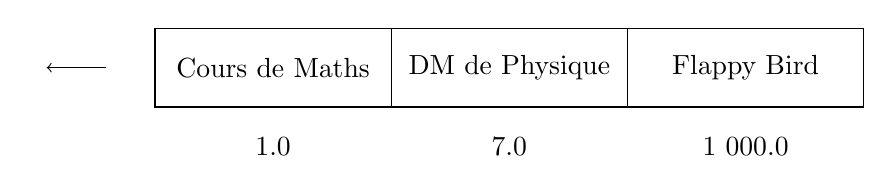
\begin{tikzpicture}
\filldraw [fill=white, draw=black] (0,0) rectangle (3,1) node[pos=.5] {Cours de Maths};
\filldraw [fill=white, draw=black] (3,0) rectangle (6,1) node[pos=.5] {DM de Physique};
\filldraw [fill=white, draw=black] (6,0) rectangle (9,1) node[pos=.5] {Flappy Bird};
\node[] at (1.5,-0.5) {1.0};
\node[] at (4.5,-0.5) {7.0};
\node[] at (7.5,-0.5) {$1\ 000.0$};
\node[] (A) at (-0.5,0.5) {};
\node[] (B) at (-1.5,0.5) {};
\draw[->] (A)--(B);
\end{tikzpicture}
\end{center}

\noindent
la flèche nous indiquant que la prochaine tâche à accomplir est de relire votre cours de
maths. Les nombres flottants placés en dessous de chaque tâche sont des priorités~: plus ce nombre
est bas, plus la tâche est prioritaire. Si vous apprenez que votre prochaine colle de
français a lieu dans trois jours, il faut vous ménager du temps
pour la préparer. Vous insérez donc cette nouvelle tâche dans la file avec une
priorité de $3.0$.  

\begin{center}
\begin{tikzpicture}
\filldraw [fill=white, draw=black] (0,0) rectangle (3,1) node[pos=.5] {Cours de Maths};
\filldraw [fill=colorLazoBlue1Light, draw=black] (3,0) rectangle (6,1) node[pos=.5] {Colle de Français};
\filldraw [fill=white, draw=black] (6,0) rectangle (9,1) node[pos=.5] {DM de Physique};
\filldraw [fill=white, draw=black] (9,0) rectangle (12,1) node[pos=.5] {Flappy Bird};
\node[] at (1.5,-0.5) {1.0};
\node[] at (4.5,-0.5) {3.0};
\node[] at (7.5,-0.5) {7.0};
\node[] at (10.5,-0.5) {$1\ 000.0$};
\node[] (A) at (-0.5,0.5) {};
\node[] (B) at (-1.5,0.5) {};
\draw[->] (A)--(B);
\end{tikzpicture}
\end{center}
Une réalisation concrète d'une file de priorité fournit donc les
fonctions suivantes~:
\begin{itemize}
\item Une fonction de création d'une file de priorité vide.
\item Une fonction déterminant si une file de priorité est vide.
\item Une fonction permettant d'enfiler un élément, accompagné d'une priorité.
\item Une fonction permettant de défiler l'élément ayant la priorité la plus basse.
\item Une fonction permettant de connaitre l'élément ayant la priorité la plus basse.
\end{itemize}
La signature d'une file de priorité d'entiers est donc~:

\begin{pythoncodeline}
pqueue_new() -> pqueue[int]
pqueue_is_empty(q: pqueue[int]) -> bool
pqueue_push(q: pqueue[int], x: int, p: float) -> NoneType
pqueue_pop(q: pqueue[int]) -> tuple[int, float]
pqueue_peek(q: pqueue[int]) -> tuple[int, float]
\end{pythoncodeline}

\begin{exoUnique}
\exo Expliquer comment implémenter une file de priorité d'entiers à l'aide d'une liste
  du tuples composés d'un entier et d'un nombre flottant.
\end{exoUnique}

\vspace{2ex}
Cette implémentation est cependant loin d'être efficace. Lorsque nous aurons besoin
d'une meilleure efficacité, nous pourrons utiliser le module \verb!heapq!.

\begin{pythoncodeline}
import heapq

filep = []                    # Pour créer une file de priorité vide
n = len(filep)                # Pour connaitre la longueur de la file
heapq.heappush(filep, (p, x)) # Pour insérer un élément x de priorité p
p, x = heapq.heappop(filep)   # Pour défiler un élément de priorité minimale
\end{pythoncodeline}

\subsection{Dictionnaire}

Un \emph{dictionnaire} présente de nombreuses similitudes avec les listes, si ce n'est qu'au lieu d'accéder aux éléments
par le biais d'un indice, on y accède par le biais d'une \emph{clé}. On crée un dictionnaire en suivant la
syntaxe \verb!{c1: v1, ..., cn: vn}! où $c_1,\ldots,c_n$ sont des clés, nécessairement deux à deux
distinctes, et $v_1,\ldots,v_n$ les valeurs qui leur sont associées. Ainsi, \verb!{}! crée un dictionnaire
vide.

\begin{pythoncode}
In [1]: prof = {"Info": "Fayard", "Maths": "Fayard", "Physique": "Villegas"}

In [2]: prof["Maths"]
Out[2]: 'Fayard'
\end{pythoncode}

Si $d$ est un dictionnaire et $c$ est une clé~:
\begin{itemize}
\item L'expression \verb!c in d! renvoie un booléen indiquant si la clé $c$ est présente dans le dictionnaire.
\item L'expression \verb!d[c]! renvoie la valeur associée à la clé si celle-ci est présente dans le dictionnaire.
\item L'instruction \verb!d[c] = v! crée une nouvelle association si la clé n'est pas présente dans le
  dictionnaire, et modifie l'association précédente sinon.
\item L'instruction \verb!del d[c]! supprime l'entrée associée à la clé $c$ dans le dictionnaire.
\item On peut enfin connaitre le nombre de clés présentes dans un
  dictionnaire avec la fonction \verb!len(d)!.
\end{itemize}

Le type d'un dictionnaire est \verb!dict!. En pratique les clés seront toutes d'un même type et les valeurs
seront aussi toutes du même type. Dans la signature des fonctions, on notera \verb!dict[str, int]! un dictionnaire
dont les clés sont des chaines de caractères et les valeurs sont des entiers.\\

Il est possible d'itérer sur les clés d'un dictionnaire avec la construction
\verb!for k in d.keys()!, mais on peut aussi directement itérer sur les clés et les
valeurs avec la construction \verb!for k, v in d.items()!. Par exemple~:
\begin{pythoncode}
In [3]: for k, v in prof.items():
   ...:     print("Le cours de", k, "est enseigné par M.",  v)
(*@\textcolor{purple}{Le cours de Info est enseigné par M. Fayard}@*)
(*@\textcolor{purple}{Le cours de Maths est enseigné par M. Fayard}@*)
(*@\textcolor{purple}{Le cours de Physique est enseigné par M. Villegas}@*)
\end{pythoncode}
Ces deux méthodes sont celles préconisées par le programme de prépa, mais il est plus naturel
en Python d'utiliser directement \verb!for k in d! qui a le même effet que
\verb!for k in d.keys()!. Le même programme s'écrit alors~:
\begin{pythoncode}
In [4]: for k in prof:
   ...:     print("Le cours de", k, "est enseigné par M.",  prof[k])
\end{pythoncode}
\vspace{2ex}
\begin{exoUnique}
\exo Écrire une fonction \verb!occ(lst: list[str]) -> dict[str, int]! renvoyant un dictionnaire \verb!d! tel
  que si \verb!s! est une chaine de caractères, \verb!d[s]! est le nombre d'occurrences de \verb!s! dans la liste
  \verb!lst!.
\end{exoUnique}
\vspace{2ex}
Il est possible de simuler un ensemble à l'aide d'un dictionnaire. Un ensemble d'entiers \verb!s! sera tout
simplement un dictionnaire \verb!dict[int, NoneType]!. On ajoutera un entier \verb!a! à cet ensemble
à l'aide de l'instruction \verb!s[a] = None! et on le supprimera avec l'instruction
\verb!del s[a]!.



%END_BOOK

\end{document}
